%----------------------------------------------------------------------------
\chapter{Jegyzőkönyv}
%----------------------------------------------------------------------------
%----------------------------------------------------------------------------
\section{Első feladat}
%----------------------------------------------------------------------------
Először definiáltunk egy mintavételi időt, amit aztán annak a megelőzésére használunk fel, hogy egy kézmozdulatot két külön mozdulatként érzékeljünk. Kezdetben ezt az értéket 150 ms-nak definiáltuk, de ez kicsinek bizonyult,  300 ms-os értékkel megfelelően robusztusan működött. Ha a két mozdulat között eltelt idő nagyobb, mint az általunk beállított limit, akkor a handlist változóba elmentjük a detektált mozdulatok listáját és továbbadjuk azt a processHands függvénynek, az utolsó detektálás idejét pedig frissítjük az aktuálisra.

\begin{lstlisting}
const double THRESHOLD_PROCESS_FRAME = 300;
clock_t this_time = clock();
clock_t last_time = this_time;
void processFrame(Frame frame) {
	this_time = clock();
	if ((this_time - last_time) > THRESHOLD_PROCESS_FRAME) {
		Leap::HandList handList = frame.hands();
		last_time = this_time;
		processHands(handList);
	}
}	
\end{lstlisting}
A processHands függvény megkapja a kezek pillanatnyi tartalmazó hands listát. Végigmenve a listán, minden elemére megvizsgáljuk, hogy az adott kéz sebessége mekkora. Ehhez a hand objektum palmVelocity metódusát használjuk, ami megadja a kéz mozgásának sebességét és irányát. Ha a mozgás sebessége 750 felett van (mm/sec), akkor swipe gesztusnak minősítjük a mozdulatot. A 750-es választással a kicsit lassabb mozdulatokat is swipe gesztusként kezeljük.

\begin{lstlisting}
void processHands(HandList hands) {
	for(int i = 0; i<hands.count();++i){
		Hand hand = hands[i];
		Leap::Vector velocity = hand.palmVelocity();
		if (velocity.magnitude() > 750)
			processSwipe(velocity, hand.isLeft());
		grabTest(hand, hand.isLeft());
	}
}
\end{lstlisting}

%----------------------------------------------------------------------------
\section{Második feladat}
%----------------------------------------------------------------------------
A függvény bemenete egy kéz pillanatnyi sebességét és annak irányát tartalmazó vektor valamint egy logikai érték arra vonatkozóan, hogy melyik kézzel történt  mozdulat. A függvény elején definiáljuk a jobb, bal, fel, le vektorokat, amelyekkel összehasonlítva a bemeneti vektort meg tudjuk állapítani annak irányát. Ezután a bemeneti vektornak minden irányvektorral bezárt szögét elmentjük a dir tömbbe, majd ezekből kiválasztjuk a legkisebb értéket, ami megadja, hogy milyen irányú volt a kézmozgás. A konzolra kiírjuk, hogy ez az érték radiánban mennyivel tér el az irányvektortól, illetve hogy melyik irányvektorhoz áll a legközelebb, és meghívjuk az annak megfelelő sendSwipe függvényt, ami a communication.hpp fájlban van definiálva.


\lstinputlisting{figures/m10/2.cpp}
\begin{figure}[!ht]
	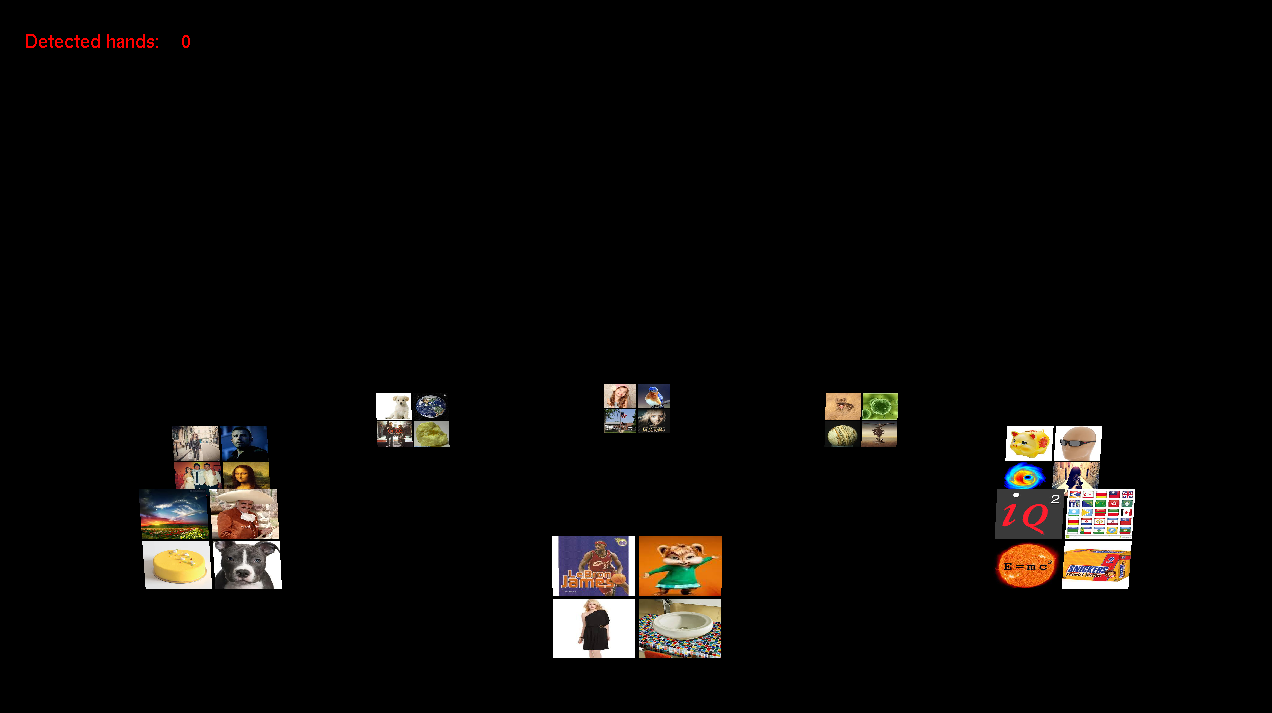
\includegraphics[width=150mm,keepaspectratio]{figures/m10/1.png}
	\label{fig:Road-of-a-char}
	\caption{Swipe left/right - váltás az elemek között}
\end{figure}
\begin{figure}[!ht]
	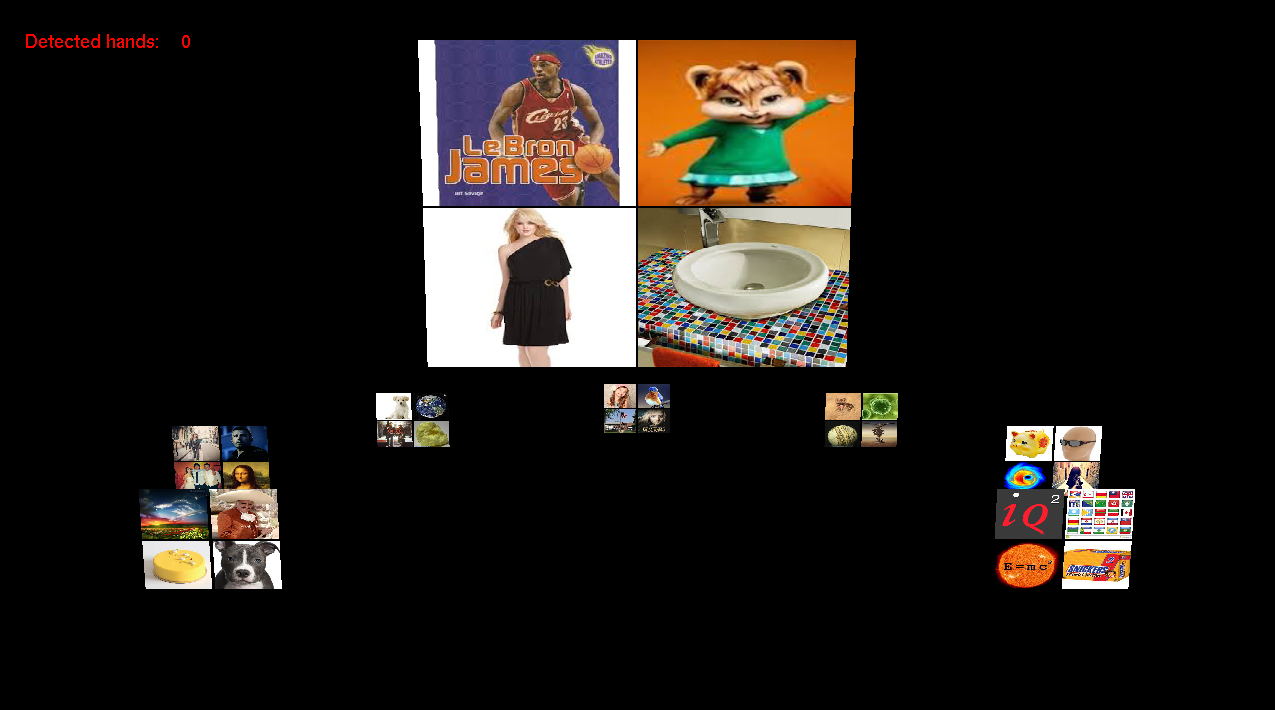
\includegraphics[width=150mm,keepaspectratio]{figures/m10/2.png}
	\caption{Swipe up - elem kiválasztása}
\end{figure}


%----------------------------------------------------------------------------
\section{Harmadik és negyedik feladat}
%----------------------------------------------------------------------------
A grabTest függvény megállapítja, hogy a kéz ökölbe van-e szorítva, illetve, hogy jobb vagy bal kéz az, illetve ennek megfelelően be- vagy kizoomolunk. Először megnézzük, hogy ökölben van-e a kéz, amit a grabStrength függvény kimenetét egy threshold értékkel összehasonlítva kapunk meg. Ha a kéz ökölben van és az előző függvényhívásnál még nem volt ökölben (isGrabLeft és isGrabRight változók), akkor zoomolonk. Megvizsgáljuk jobb és bal kézre is, az határozza meg, hogy ki- vagy bezoomolás történik. Ezt a konzolra is kiírjuk.

\lstinputlisting{figures/m10/3-4.cpp}
\begin{figure}[!ht]
	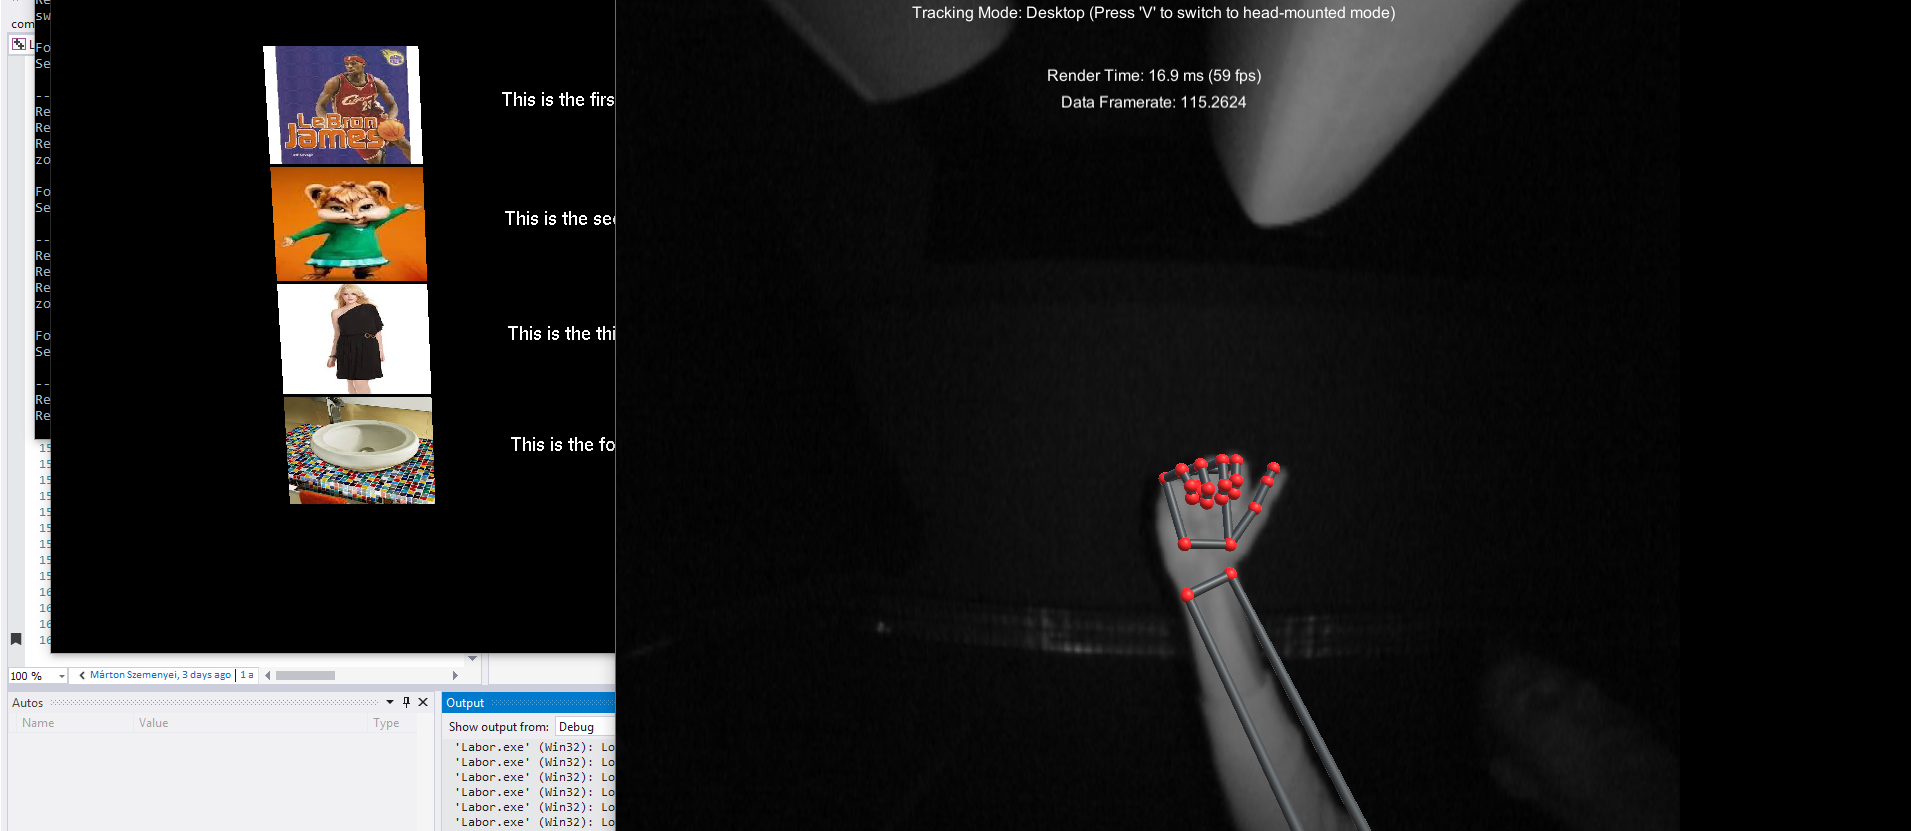
\includegraphics[width=150mm,keepaspectratio]{figures/m10/3.png}
	\caption{Zoomolás ökölbe szorításra}
\end{figure}

%----------------------------------------------------------------------------
\section{Ötödik feladat}
%----------------------------------------------------------------------------
Az előző feladatban megírt függvényt módosítjuk ehhez a feladathoz. A grab\_counter változóban számoljuk a kattintások számát. Ha ökölbe szorítás történik, növeljük a változó értékét és elmentjük a hozzá tartozó időpontot. Ezután megvizsgáljuk, hogy a két kattintás között eltelt idő nagyobb-e az általunk beállított limitnél. Mi ezt a threshold-ot 800 ms-ra állítottuk. Ha nagyobb, és egy grab\_counter értéke 1 bezoomolunk, ha 2 vagy több (default), akkor kizoomolunk, és ezt ki is írjuk a konzolra. A threshold idő leteltével a grab\_counter változót mindenképp nullázzuk, hogy egy későbbi kattintás ismét megjelölhesse a dupla kattintáshoz rendelkezésre álló időablak kezdetét.


\lstinputlisting{figures/m10/5.cpp}
\begin{figure}[!ht]
	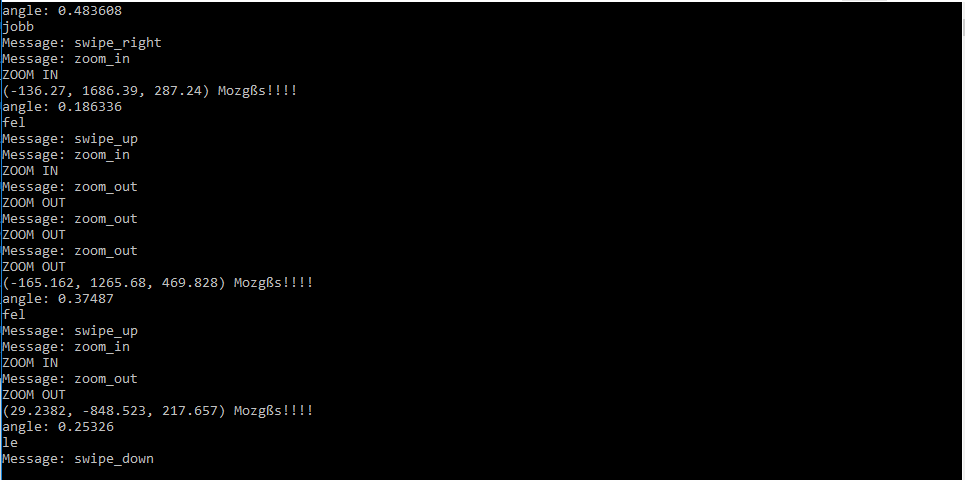
\includegraphics[width=150mm,keepaspectratio]{figures/m10/4.png}
	\caption{A konzol a rá kiírt információkkal, több egymás utáni, különböző kézmozdulat esetén.}
\end{figure}



























